\chapter{Communication in the Swarm}

\paragraph*{}
Swarm communication has been successfully implemented using a \textbf{peer-to-peer socket communication model}, where each robot can directly exchange data with others without relying on a centralized server. This architecture was chosen for its low-latency characteristics, which are crucial for real-time robotic coordination. While raw socket communication is common, the peer-to-peer topology enables direct robot-to-robot interaction, reducing delays caused by intermediaries. To improve reliability, our implementation includes connection checks, retry logic, and structured messaging formats to ensure data integrity. Within the swarm, this communication setup allows continuous exchange of positional data for effective self-collision avoidance and enables robots to relay relevant information to the designated taskmaster for path planning. The overall communication flow is illustrated in Figure \ref{fig:communication-flow}.

\begin{figure}
    \centering
    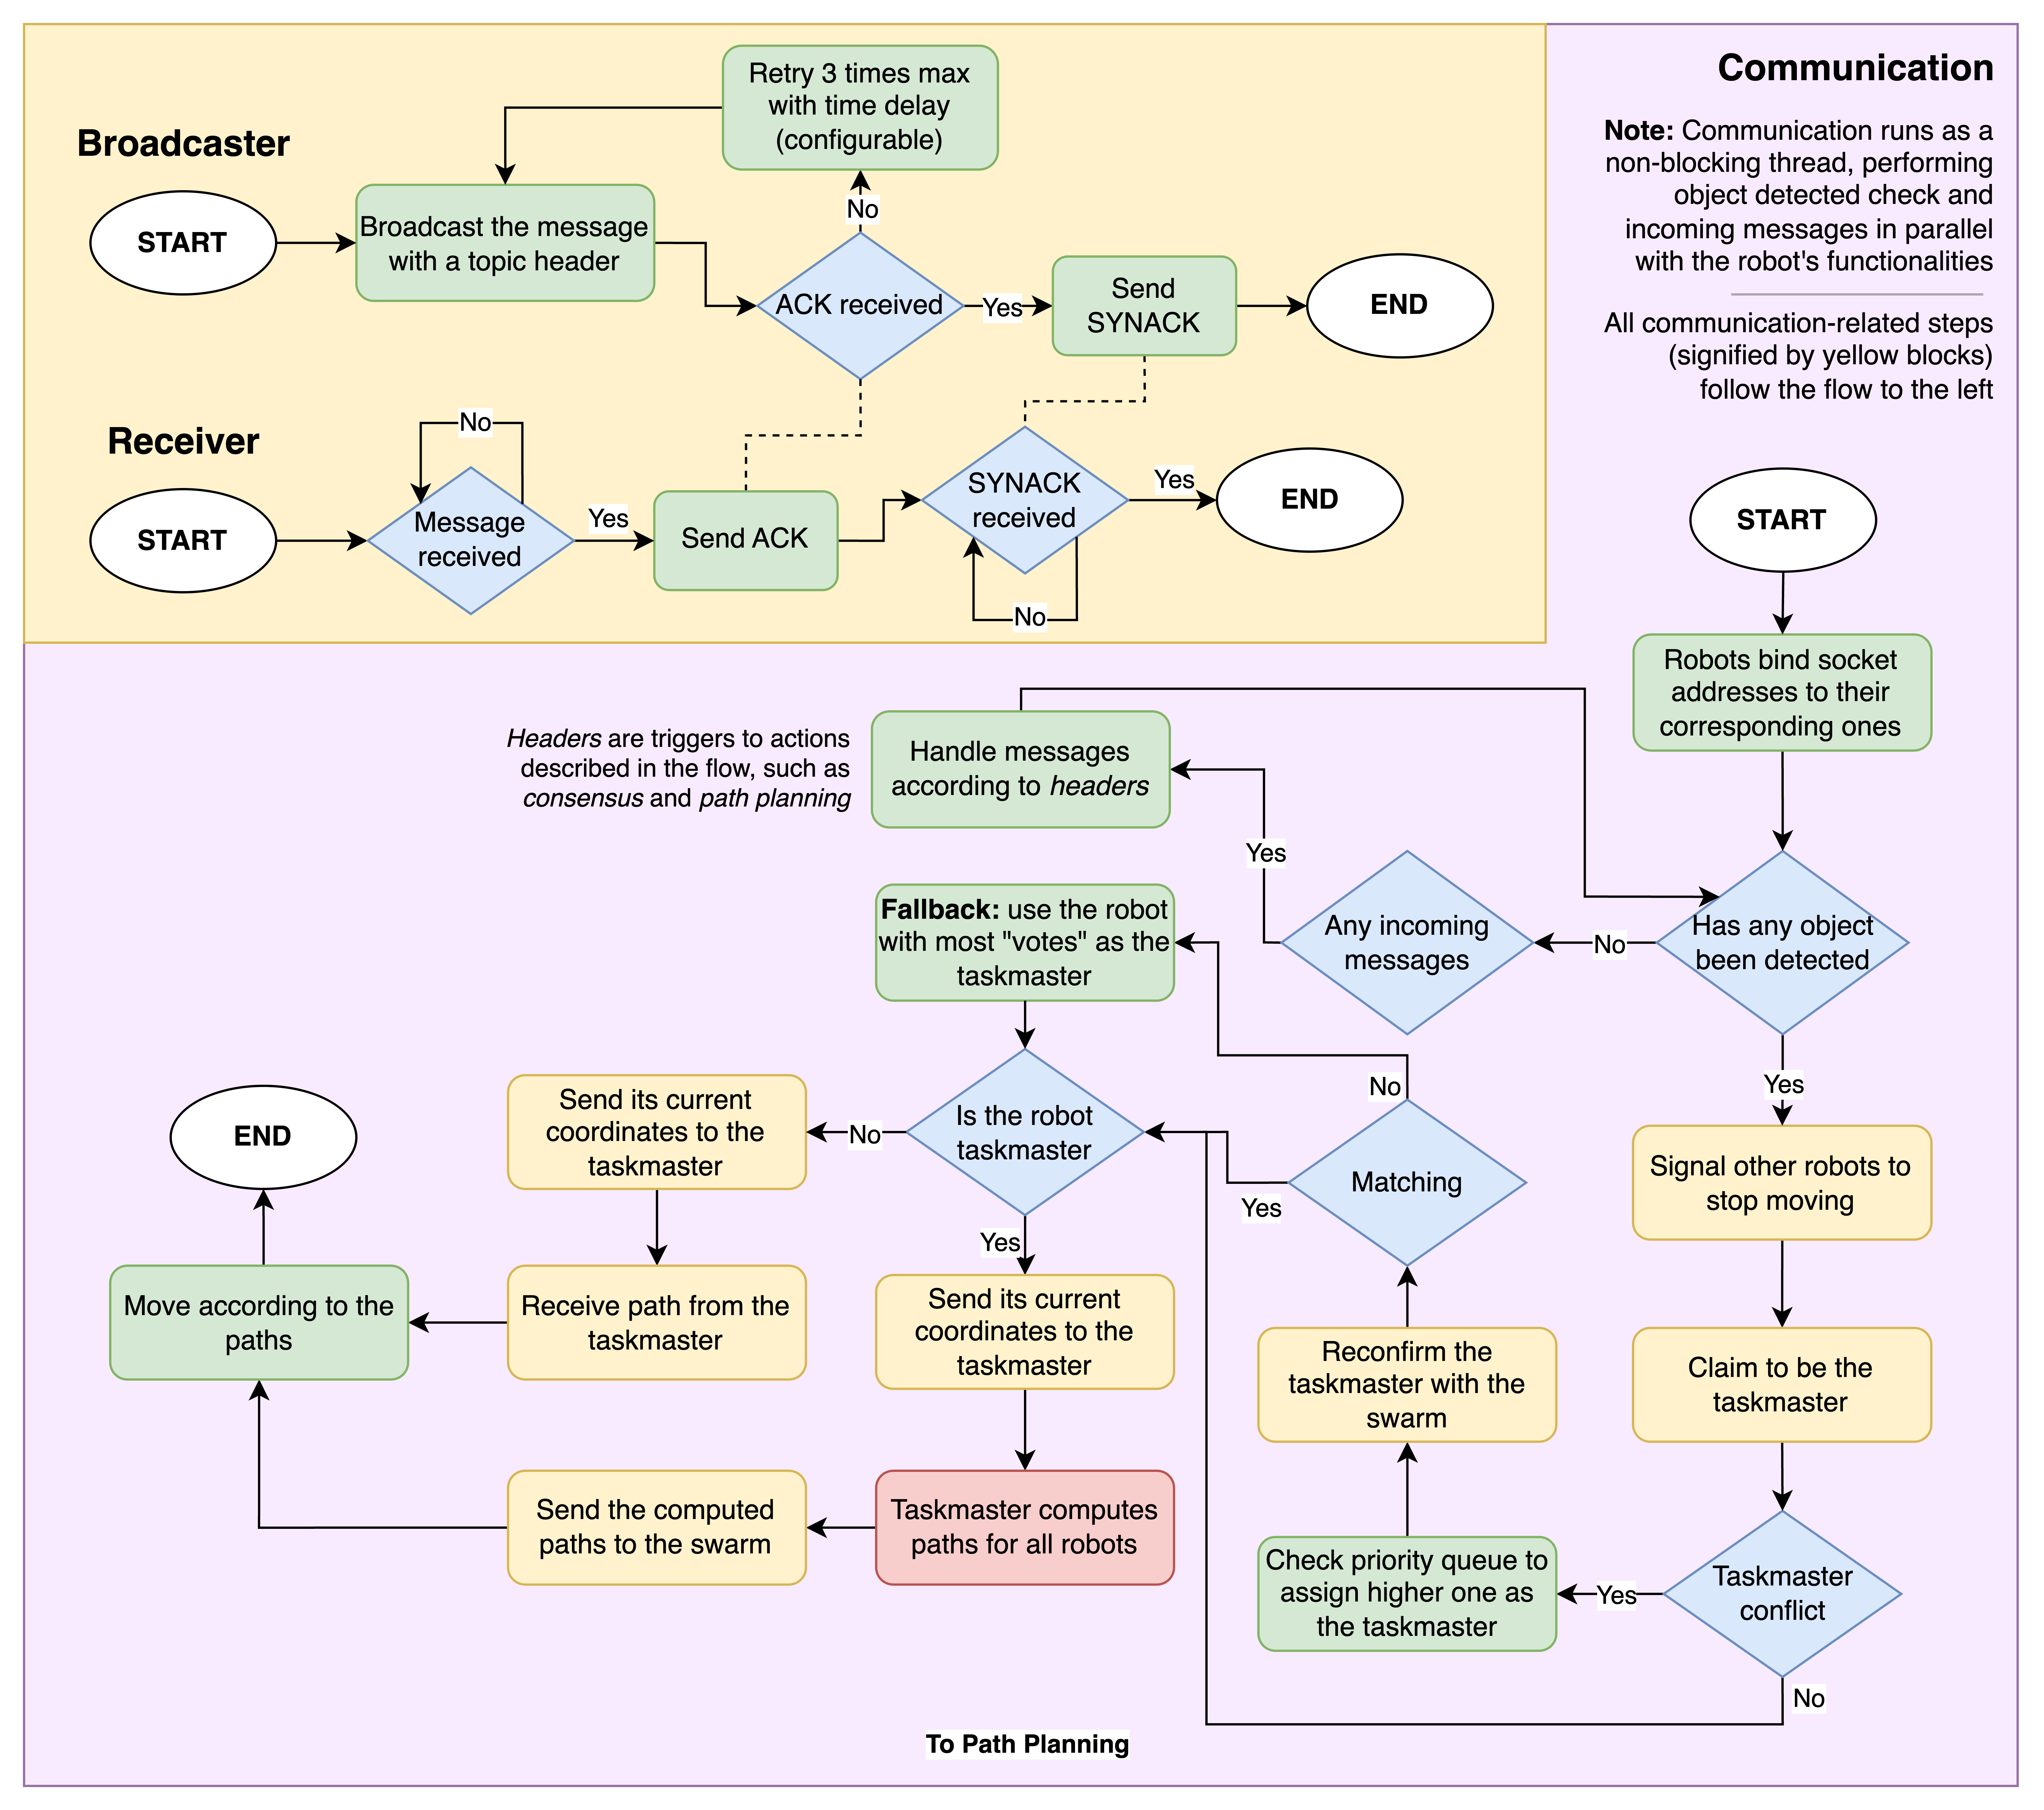
\includegraphics[width=1\linewidth]{assets/images/communication/communication-flow.png}
    \caption{Communication in the Swarm Detailed Flow}
    \label{fig:communication-flow}
\end{figure}

\paragraph*{}
There are two main implementations using communication mechanism in the swarm. The implementations are the \textbf{"constant coordinate stream"}, and the \textbf{"swarm detection task flow"}. For simplicity, all future descriptions of the communication mechanism will refer to the robots as \textit{"Robot A"}, \textit{"Robot B"} and \textit{"Robot C"}.

\paragraph*{}
The \textbf{constant coordinate stream} is a stream of coordinates in a fixed, configurable interval between the robots A, B, and C. They share their current X and Y positions with one another, updated by data obtained from the odometry. It is essential for the robots in the swarm to know the positions of one another so the movement controller will allow them roam in a collision-free manner. Figure \ref{fig:coordinate-stream} is a simple display of the constant coordinate stream in action, providing an overview to the data the robots will obtain from this coordinate stream. The output is obtained from Robot B, where it is able to continuously track the coordinates of Robot A, Robot C, as well as itself, even with the others' coordinates being updated from their respective movements.

\begin{figure} [H]
    \centering
    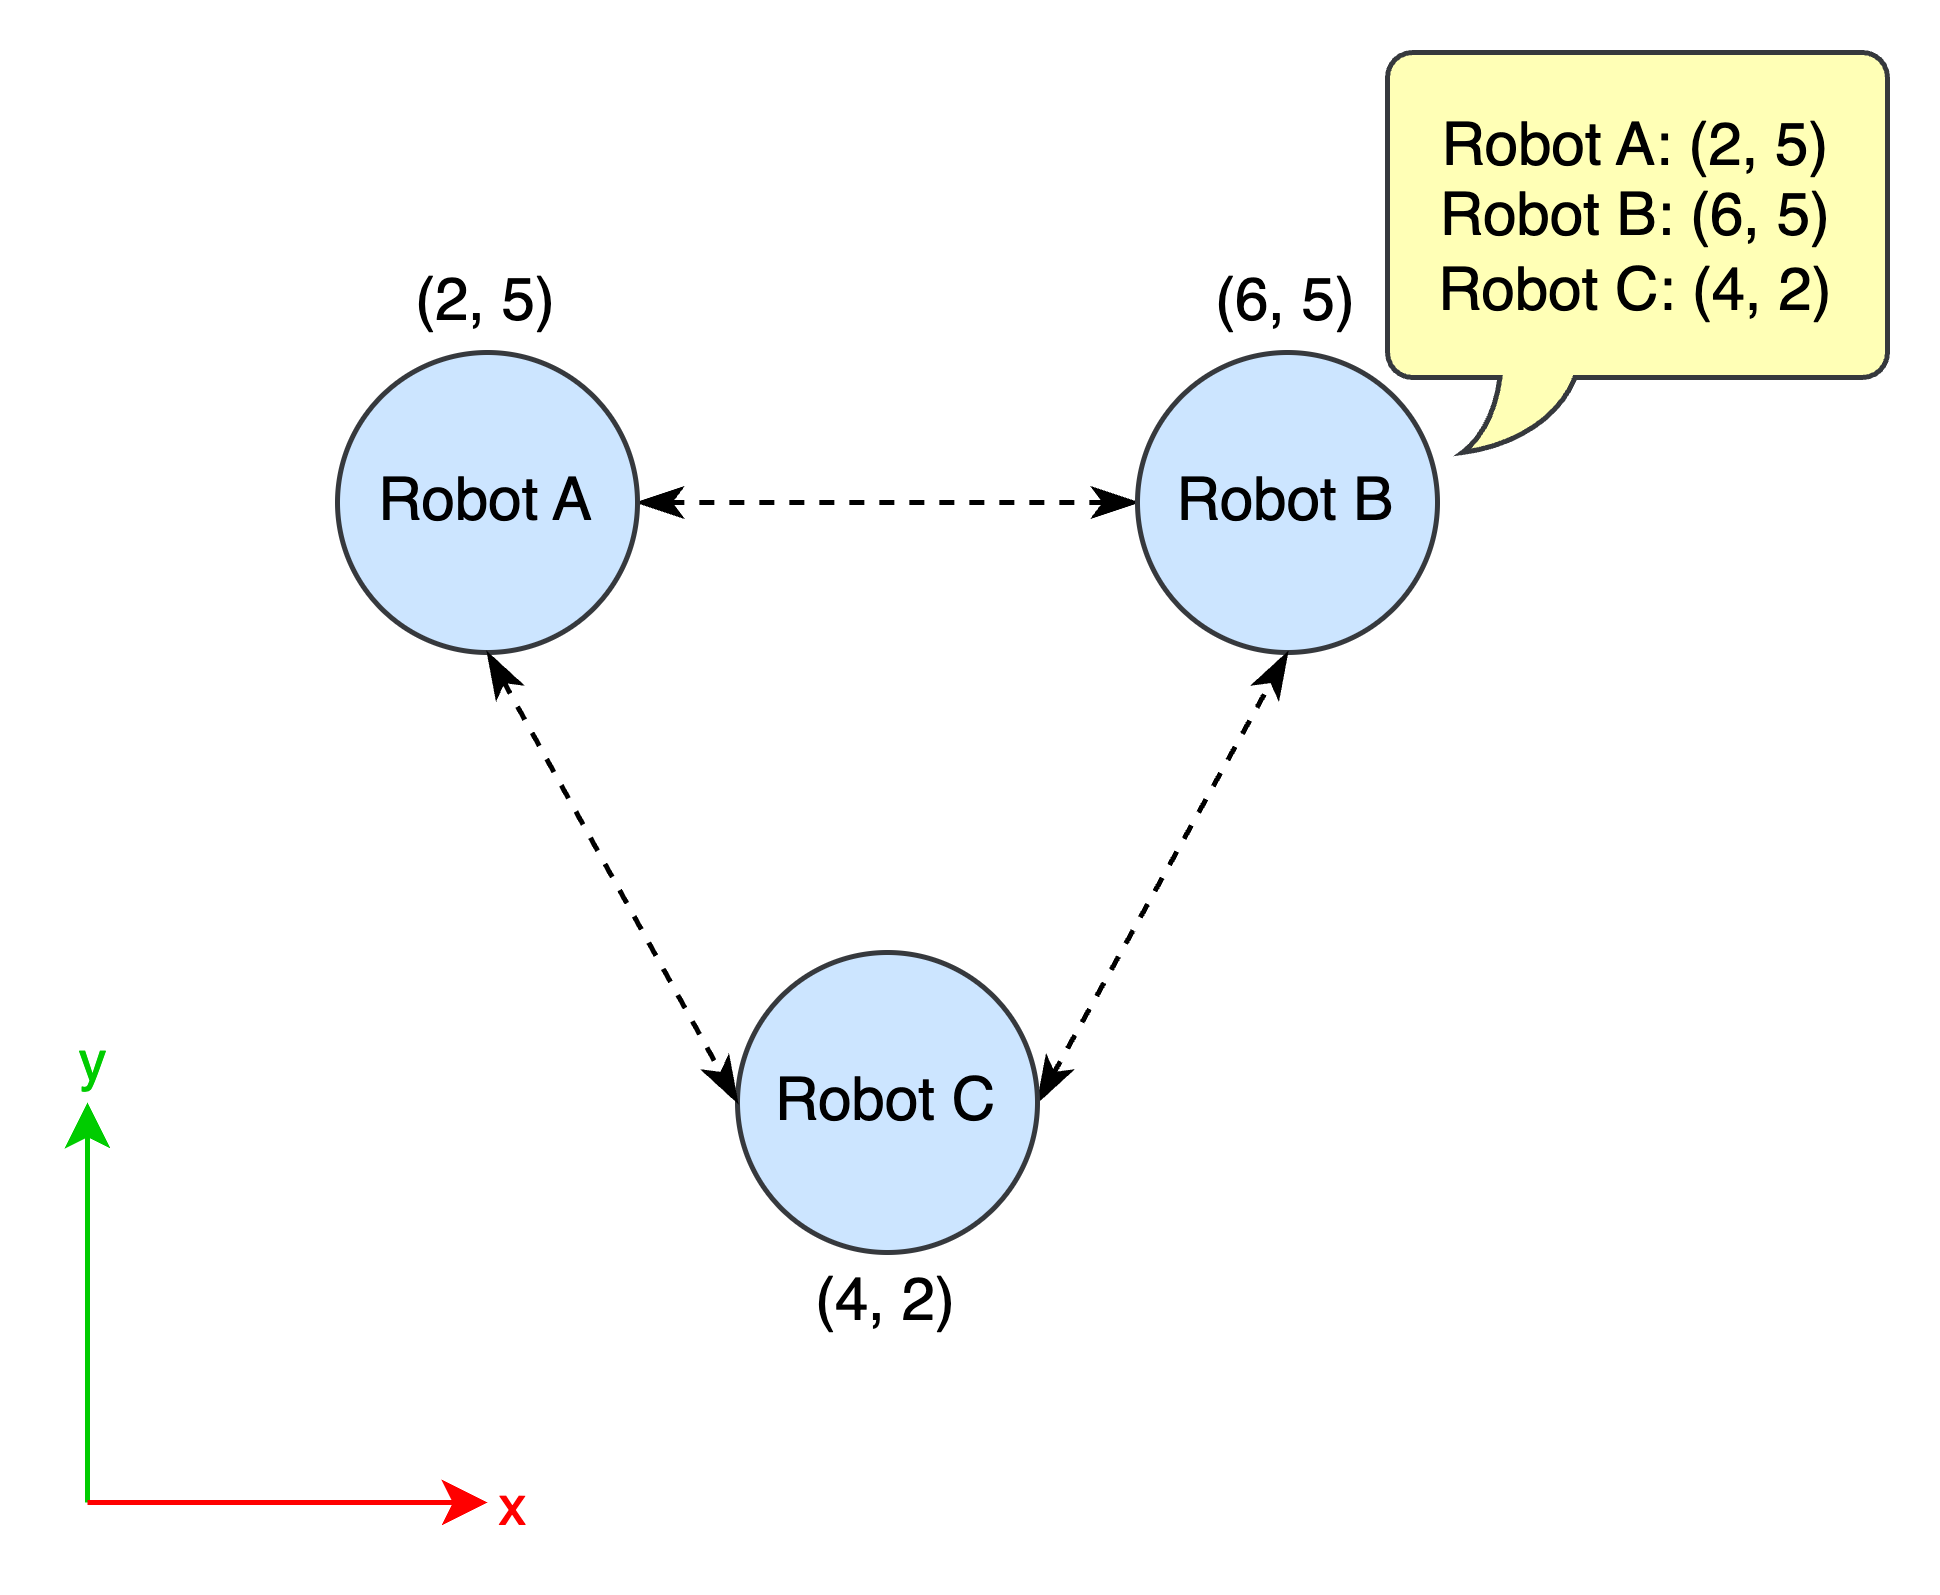
\includegraphics[width=0.6\linewidth]{assets/images/communication/constant-coordinate-stream.png}
    \caption{Constant Coordinate Stream}
    \label{fig:coordinate-stream}
\end{figure}

\paragraph*{}
The other essential communication implementation is the \textbf{swarm detection task flow}. When an object gets detected by the robot's object detection, the detecting robot will send a signal to the other two robots to stop moving. Figure \ref{fig:swarm-detection-task-0} illustrates an instance where Robot A detects an object and claims to be the taskmaster. Robot B and Robot C will receive a signal to stop ongoing movement (Figure \ref{fig:swarm-detection-task-1}) and await a collisionless path to move towards the object by the swarm's path planning algorithm, detailed in a later chapter.

\begin{figure} [H]
    \centering
    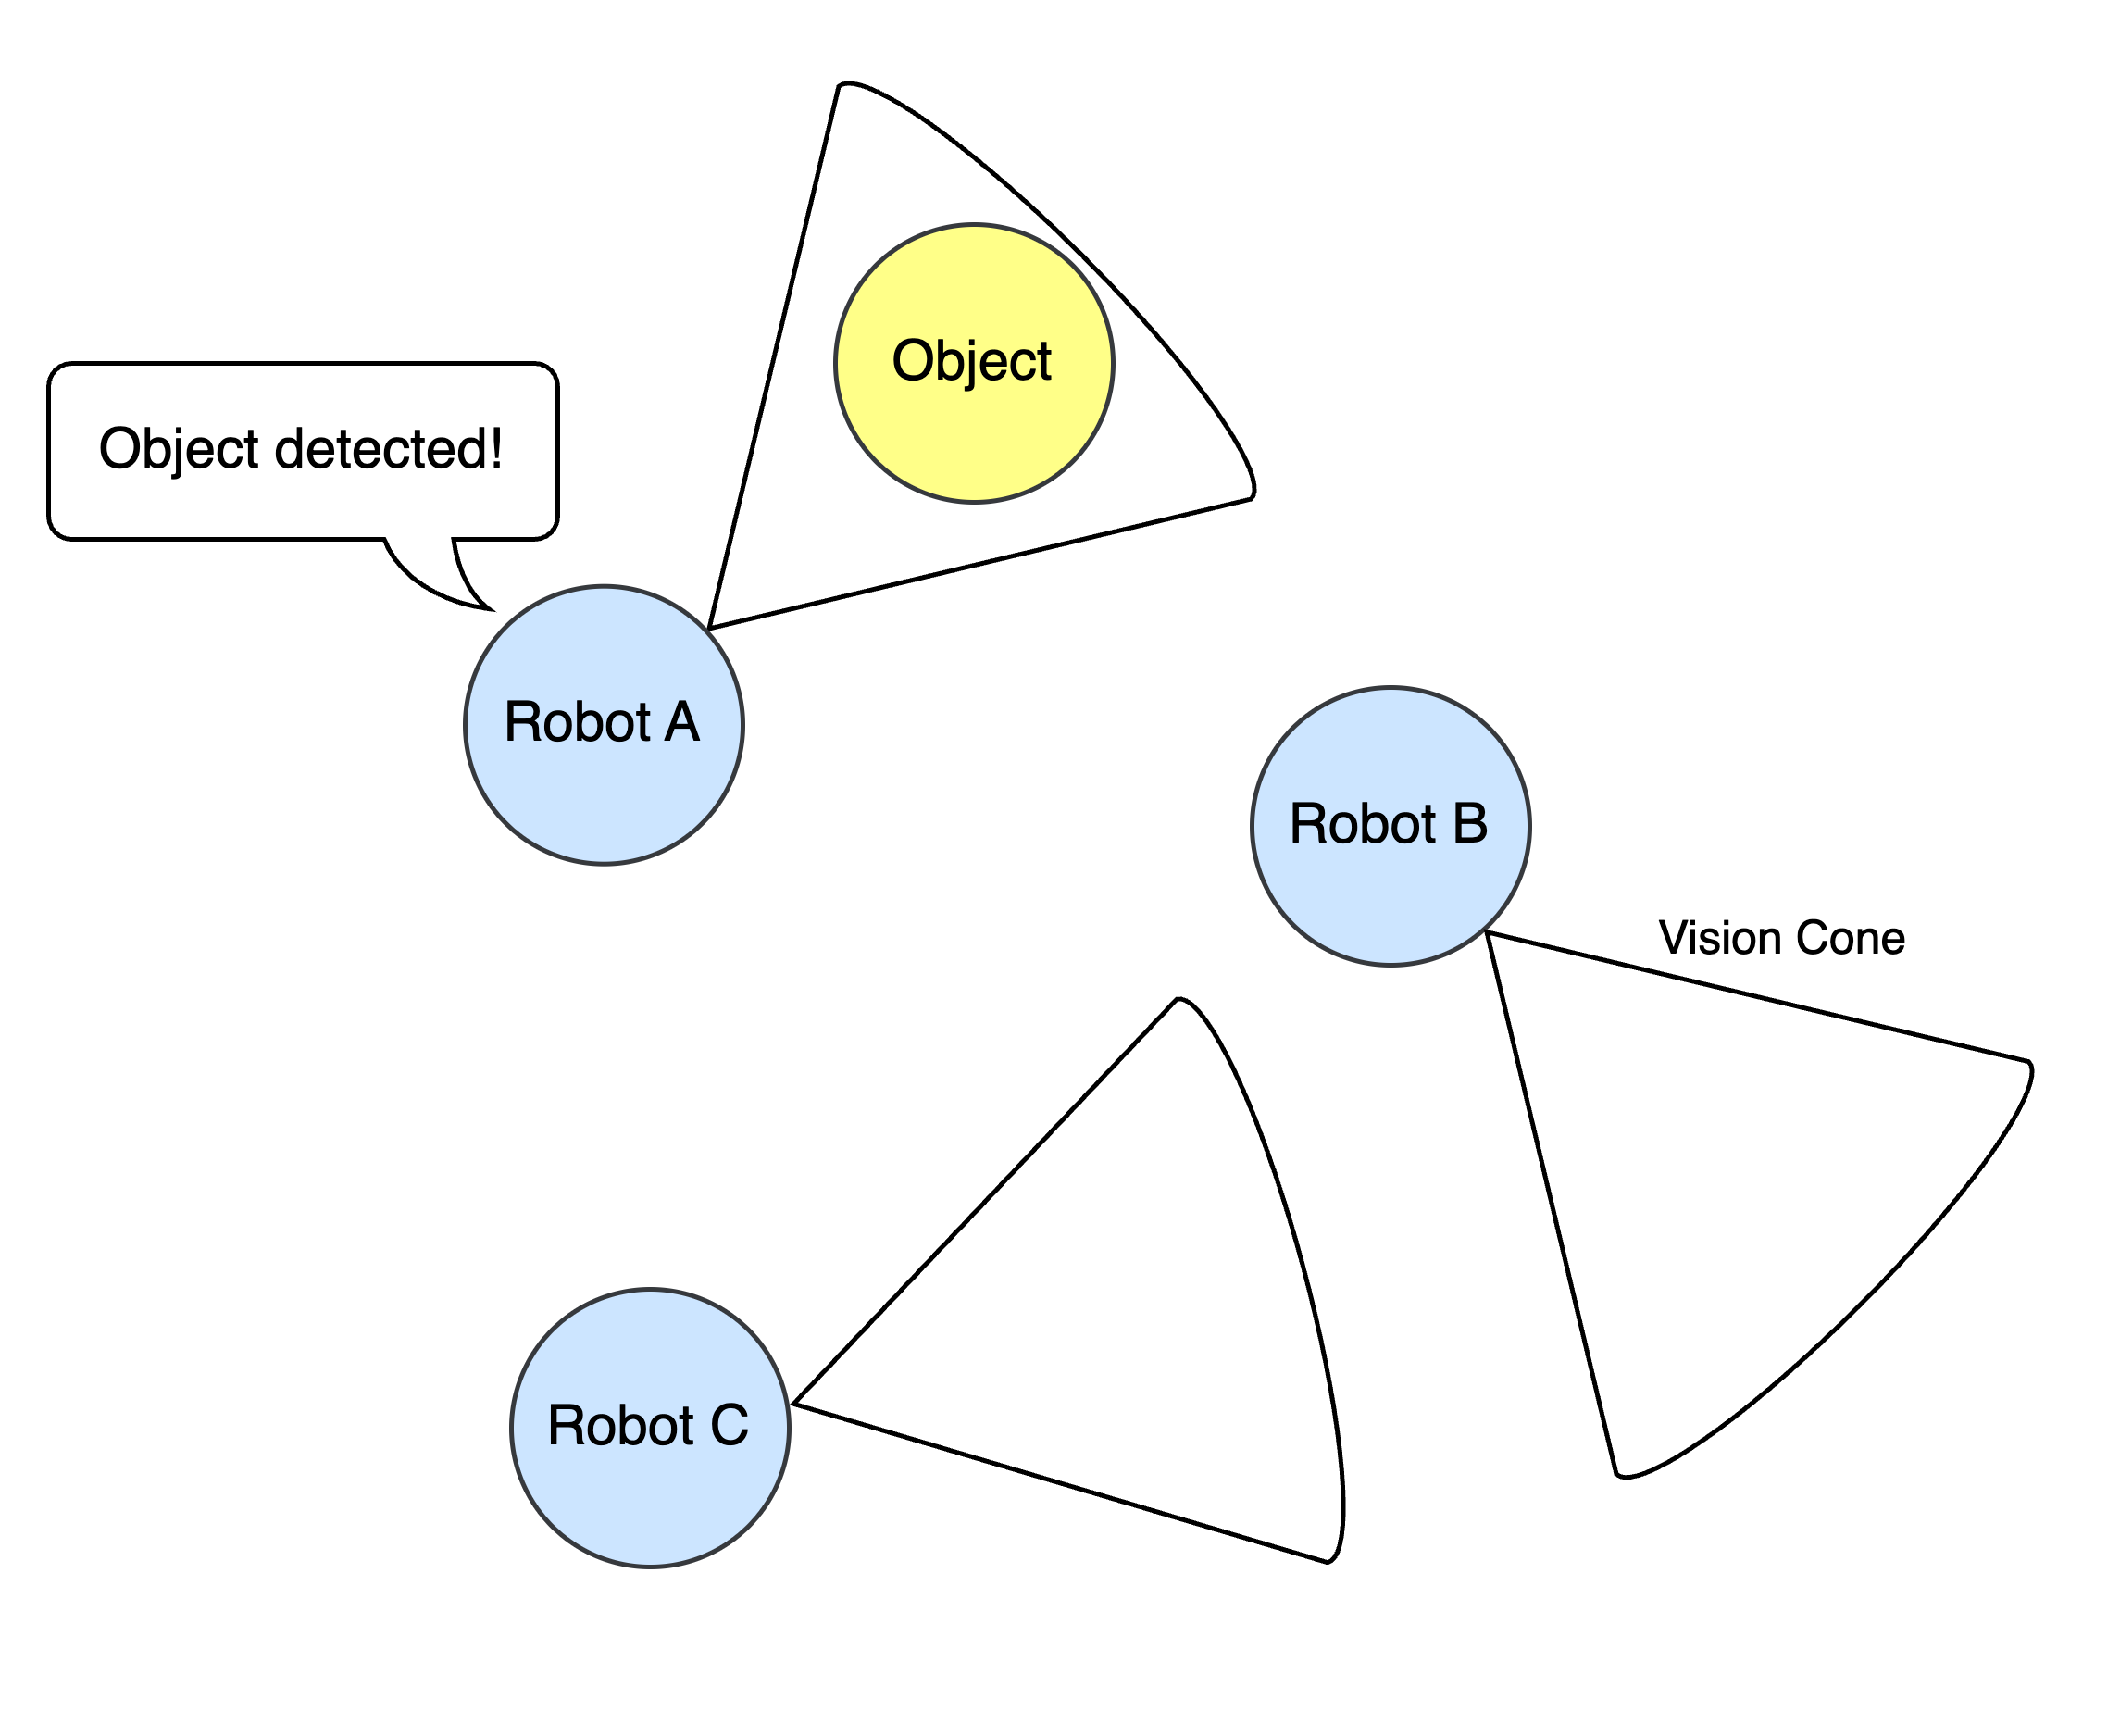
\includegraphics[width=0.6\linewidth]{assets/images/communication/swarm-detection-task-flow-0.png}
    \caption{Swarm Detection Task Flow -- Stage 0}
    \label{fig:swarm-detection-task-0}
\end{figure}

\begin{figure} [H]
    \centering
    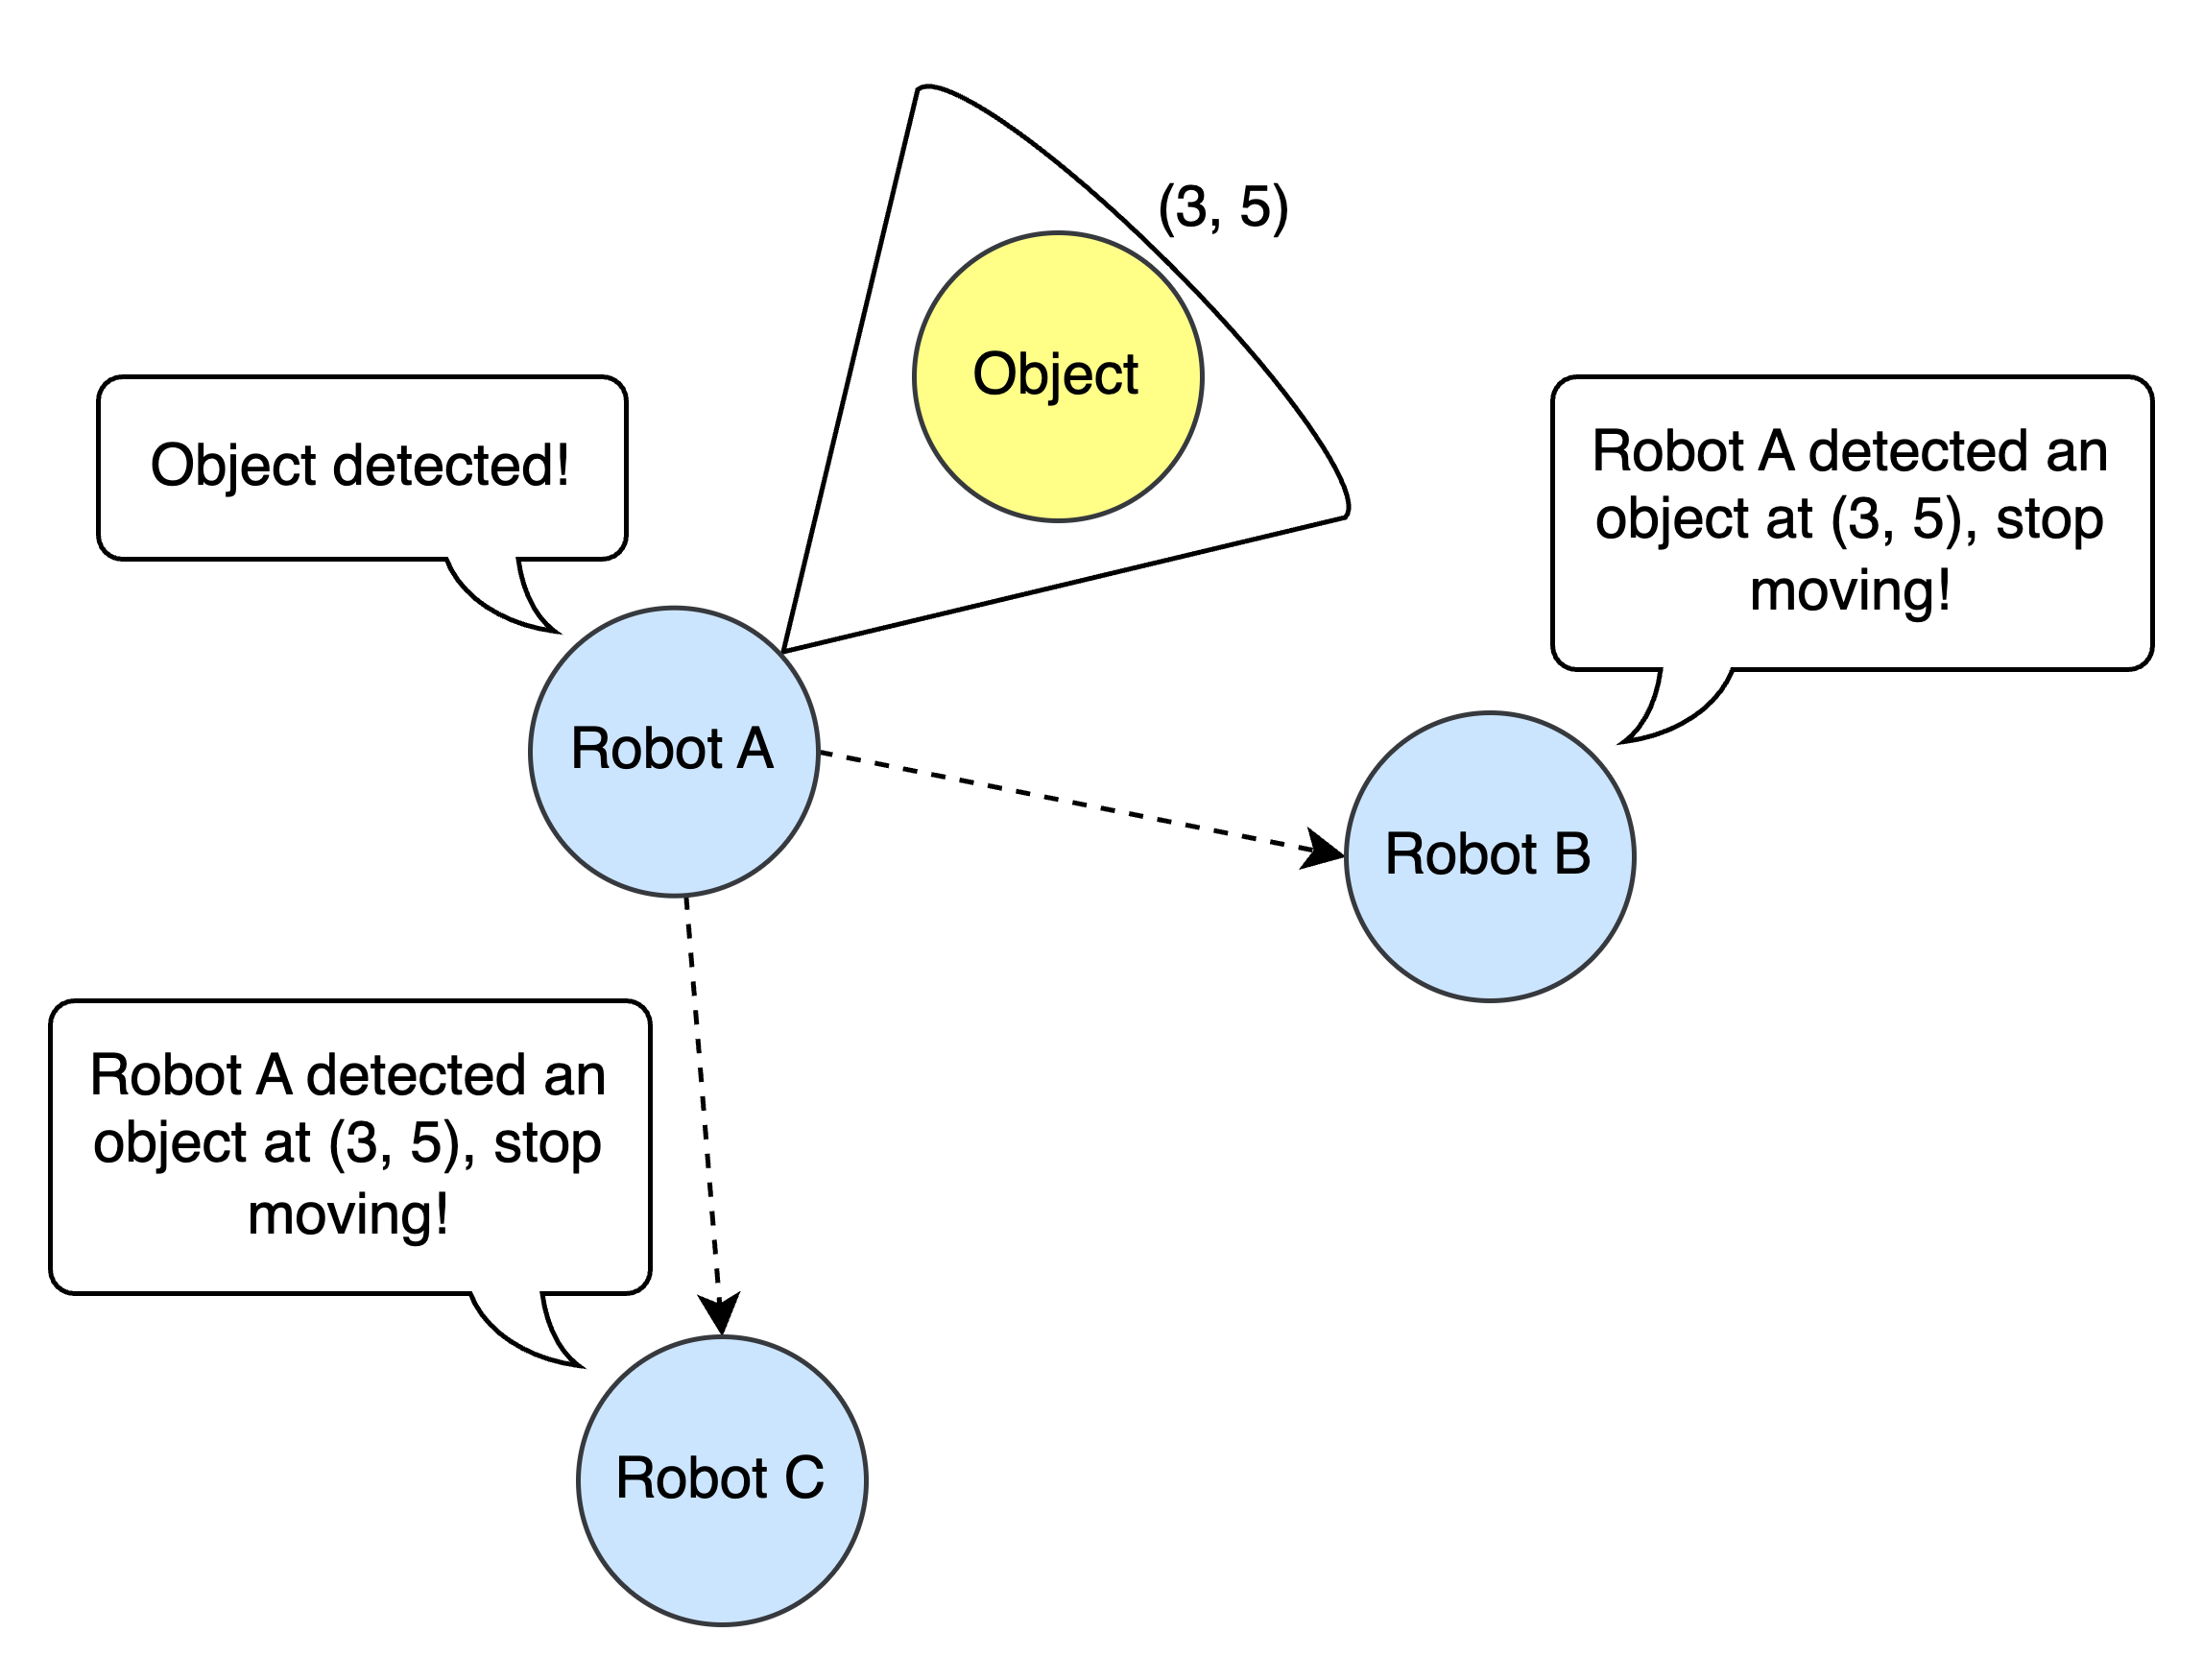
\includegraphics[width=0.6\linewidth]{assets/images/communication/swarm-detection-task-flow-1.png}
    \caption{Swarm Detection Task Flow -- Stage 1}
    \label{fig:swarm-detection-task-1}
\end{figure}

\paragraph*{}
The taskmaster, in this case, Robot A, will request current coordinates from Robot B and Robot C (Figure \ref{fig:swarm-detection-task-2}), then trigger the path planning algorithm for a set of collisionless paths for each robot. Once the set of paths are computed by the taskmaster, it will subsequently broadcast them towards others the swarm. In this case, Robot A performs the computation and broadcasts to Robot B and Robot C, allowing all of them to have their respective determined paths to move towards the detected object (Figure \ref{fig:swarm-detection-task-3})

\begin{figure} [H]
    \centering
    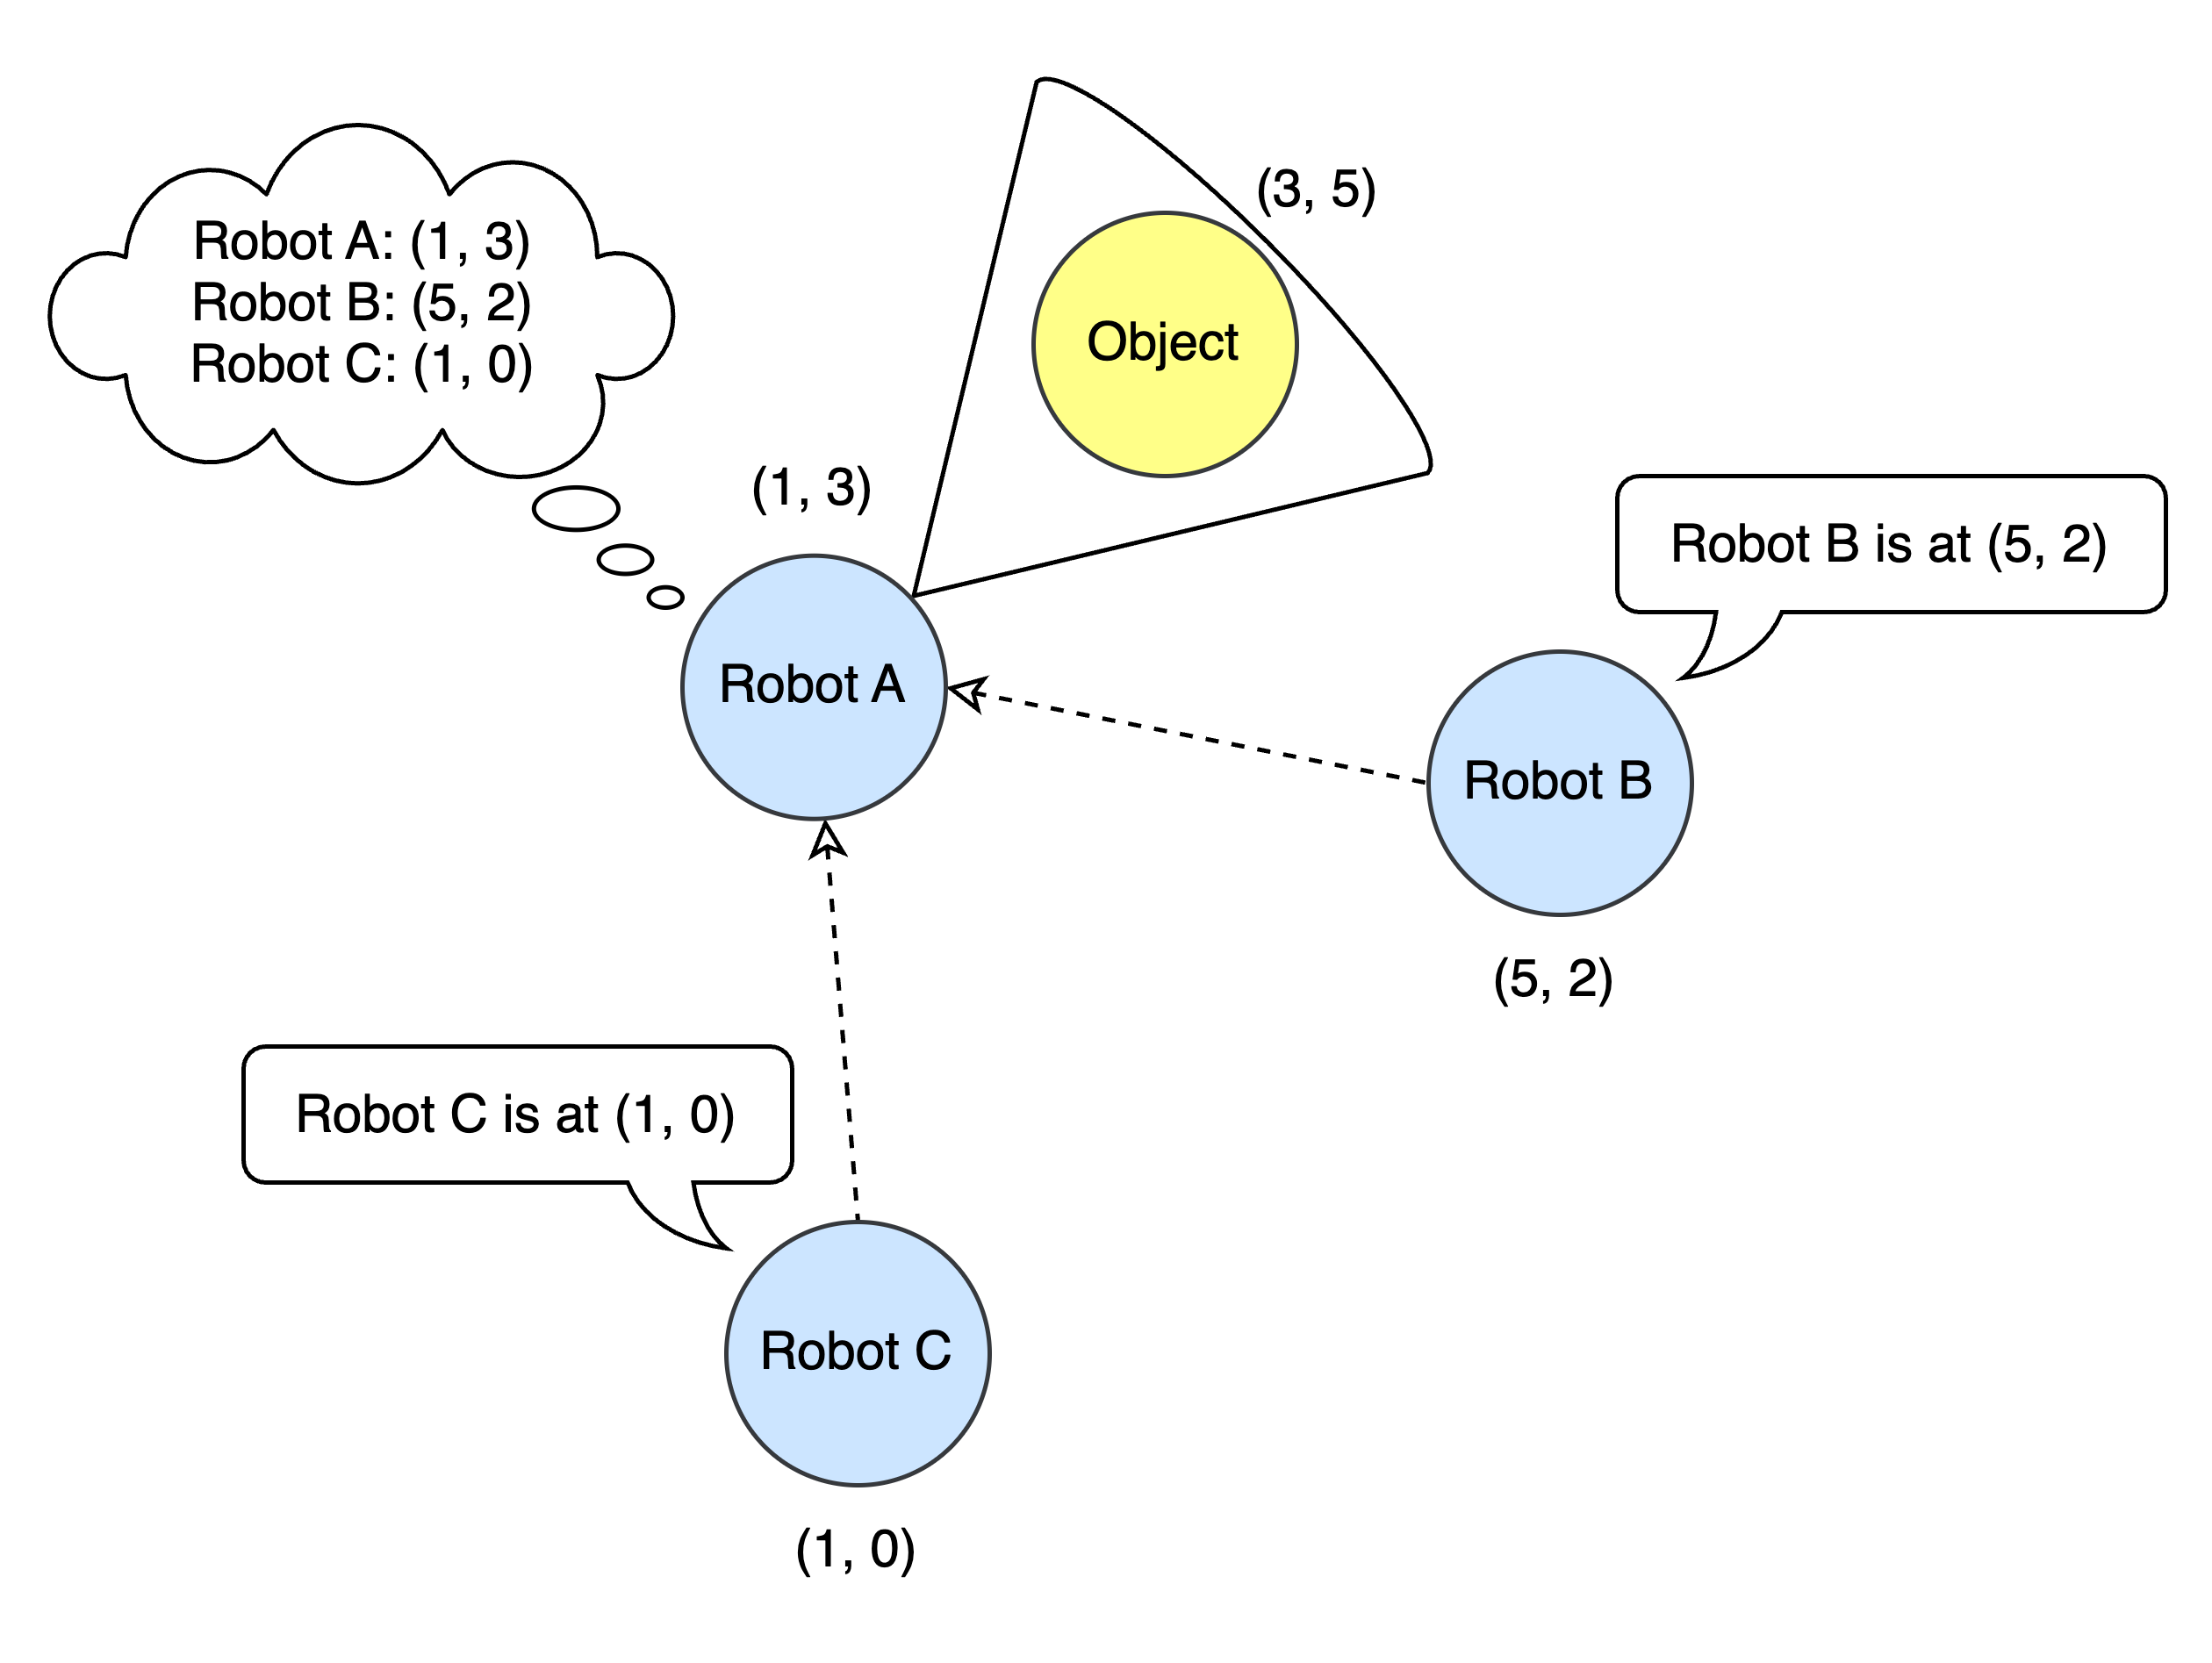
\includegraphics[width=0.6\linewidth]{assets/images/communication/swarm-detection-task-flow-2.png}
    \caption{Swarm Detection Task Flow -- Stage 2}
    \label{fig:swarm-detection-task-2}
\end{figure}

\begin{figure} [H]
    \centering
    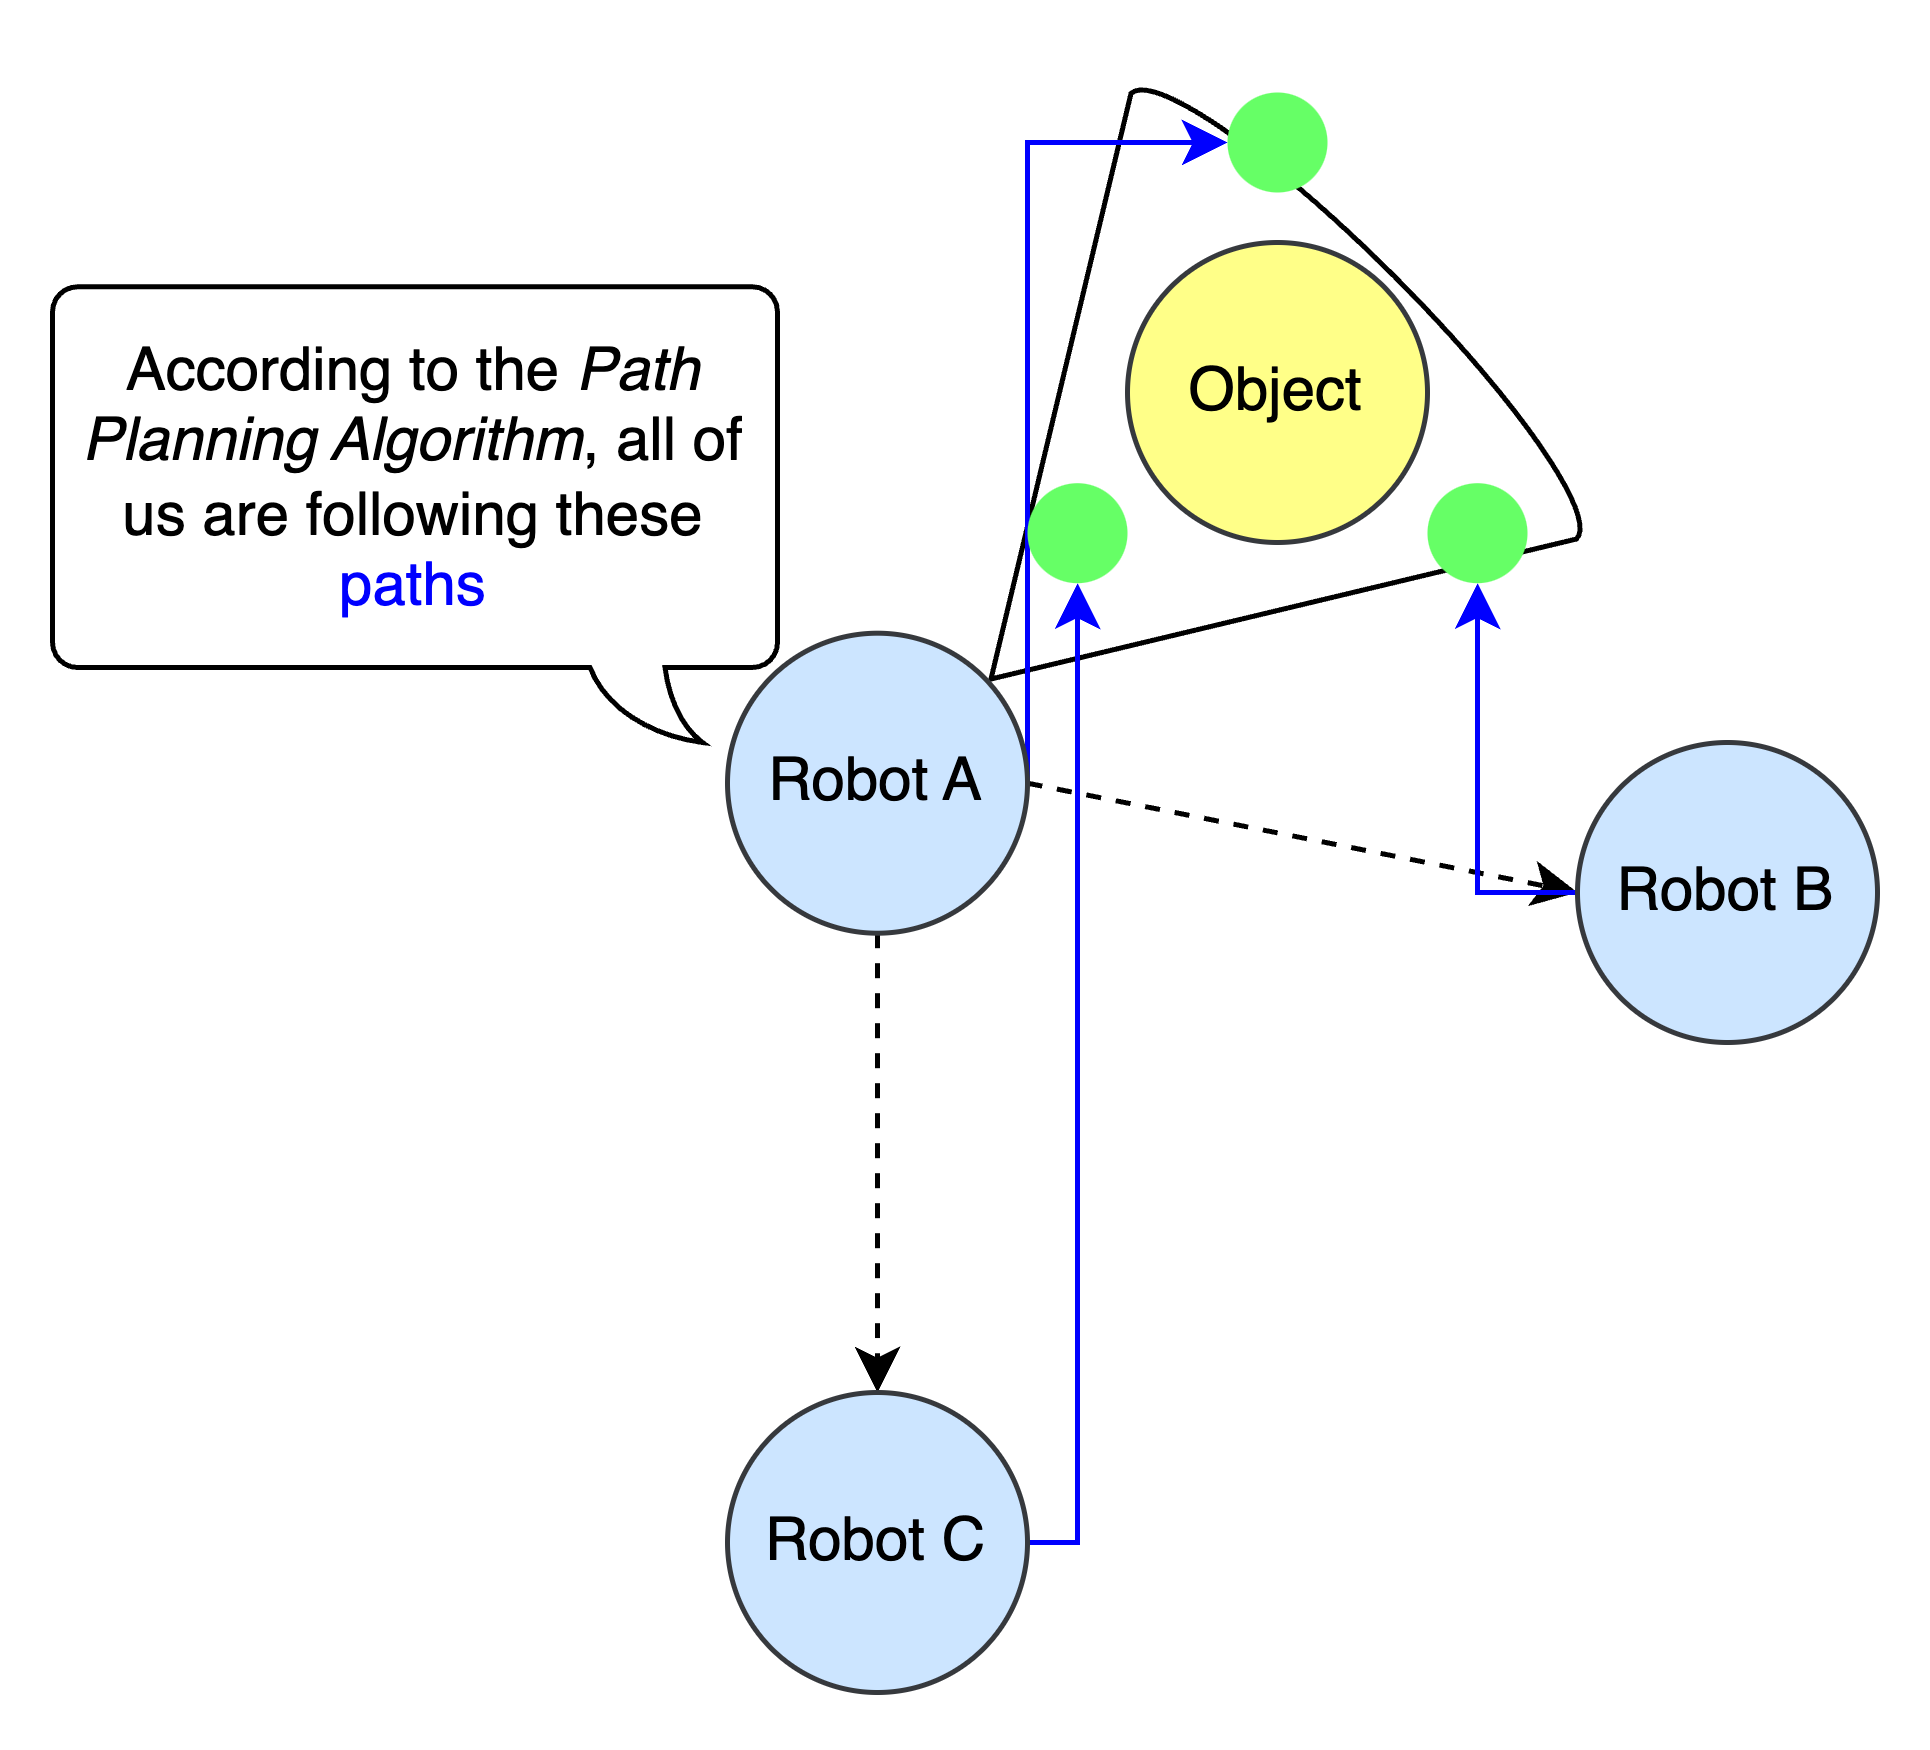
\includegraphics[width=0.6\linewidth]{assets/images/communication/swarm-detection-task-flow-3.png}
    \caption{Swarm Detection Task Flow -- Stage 3}
    \label{fig:swarm-detection-task-3}
\end{figure}

\paragraph*{}
Another thing to note is that any swarm member can become the taskmaster and perform the computations according to the \textit{swarm detection task flow}. In the described scenario, Robot A is the member that detect the object and became the taskmaster. If Robot B or Robot C were to detect the object first, they can also claim to become the taskmaster and computational lead of the swarm detection task flow. This is designed to enhance the versatility in the communication mechanism of the swarm. 

\begin{figure} [H]
    \centering
    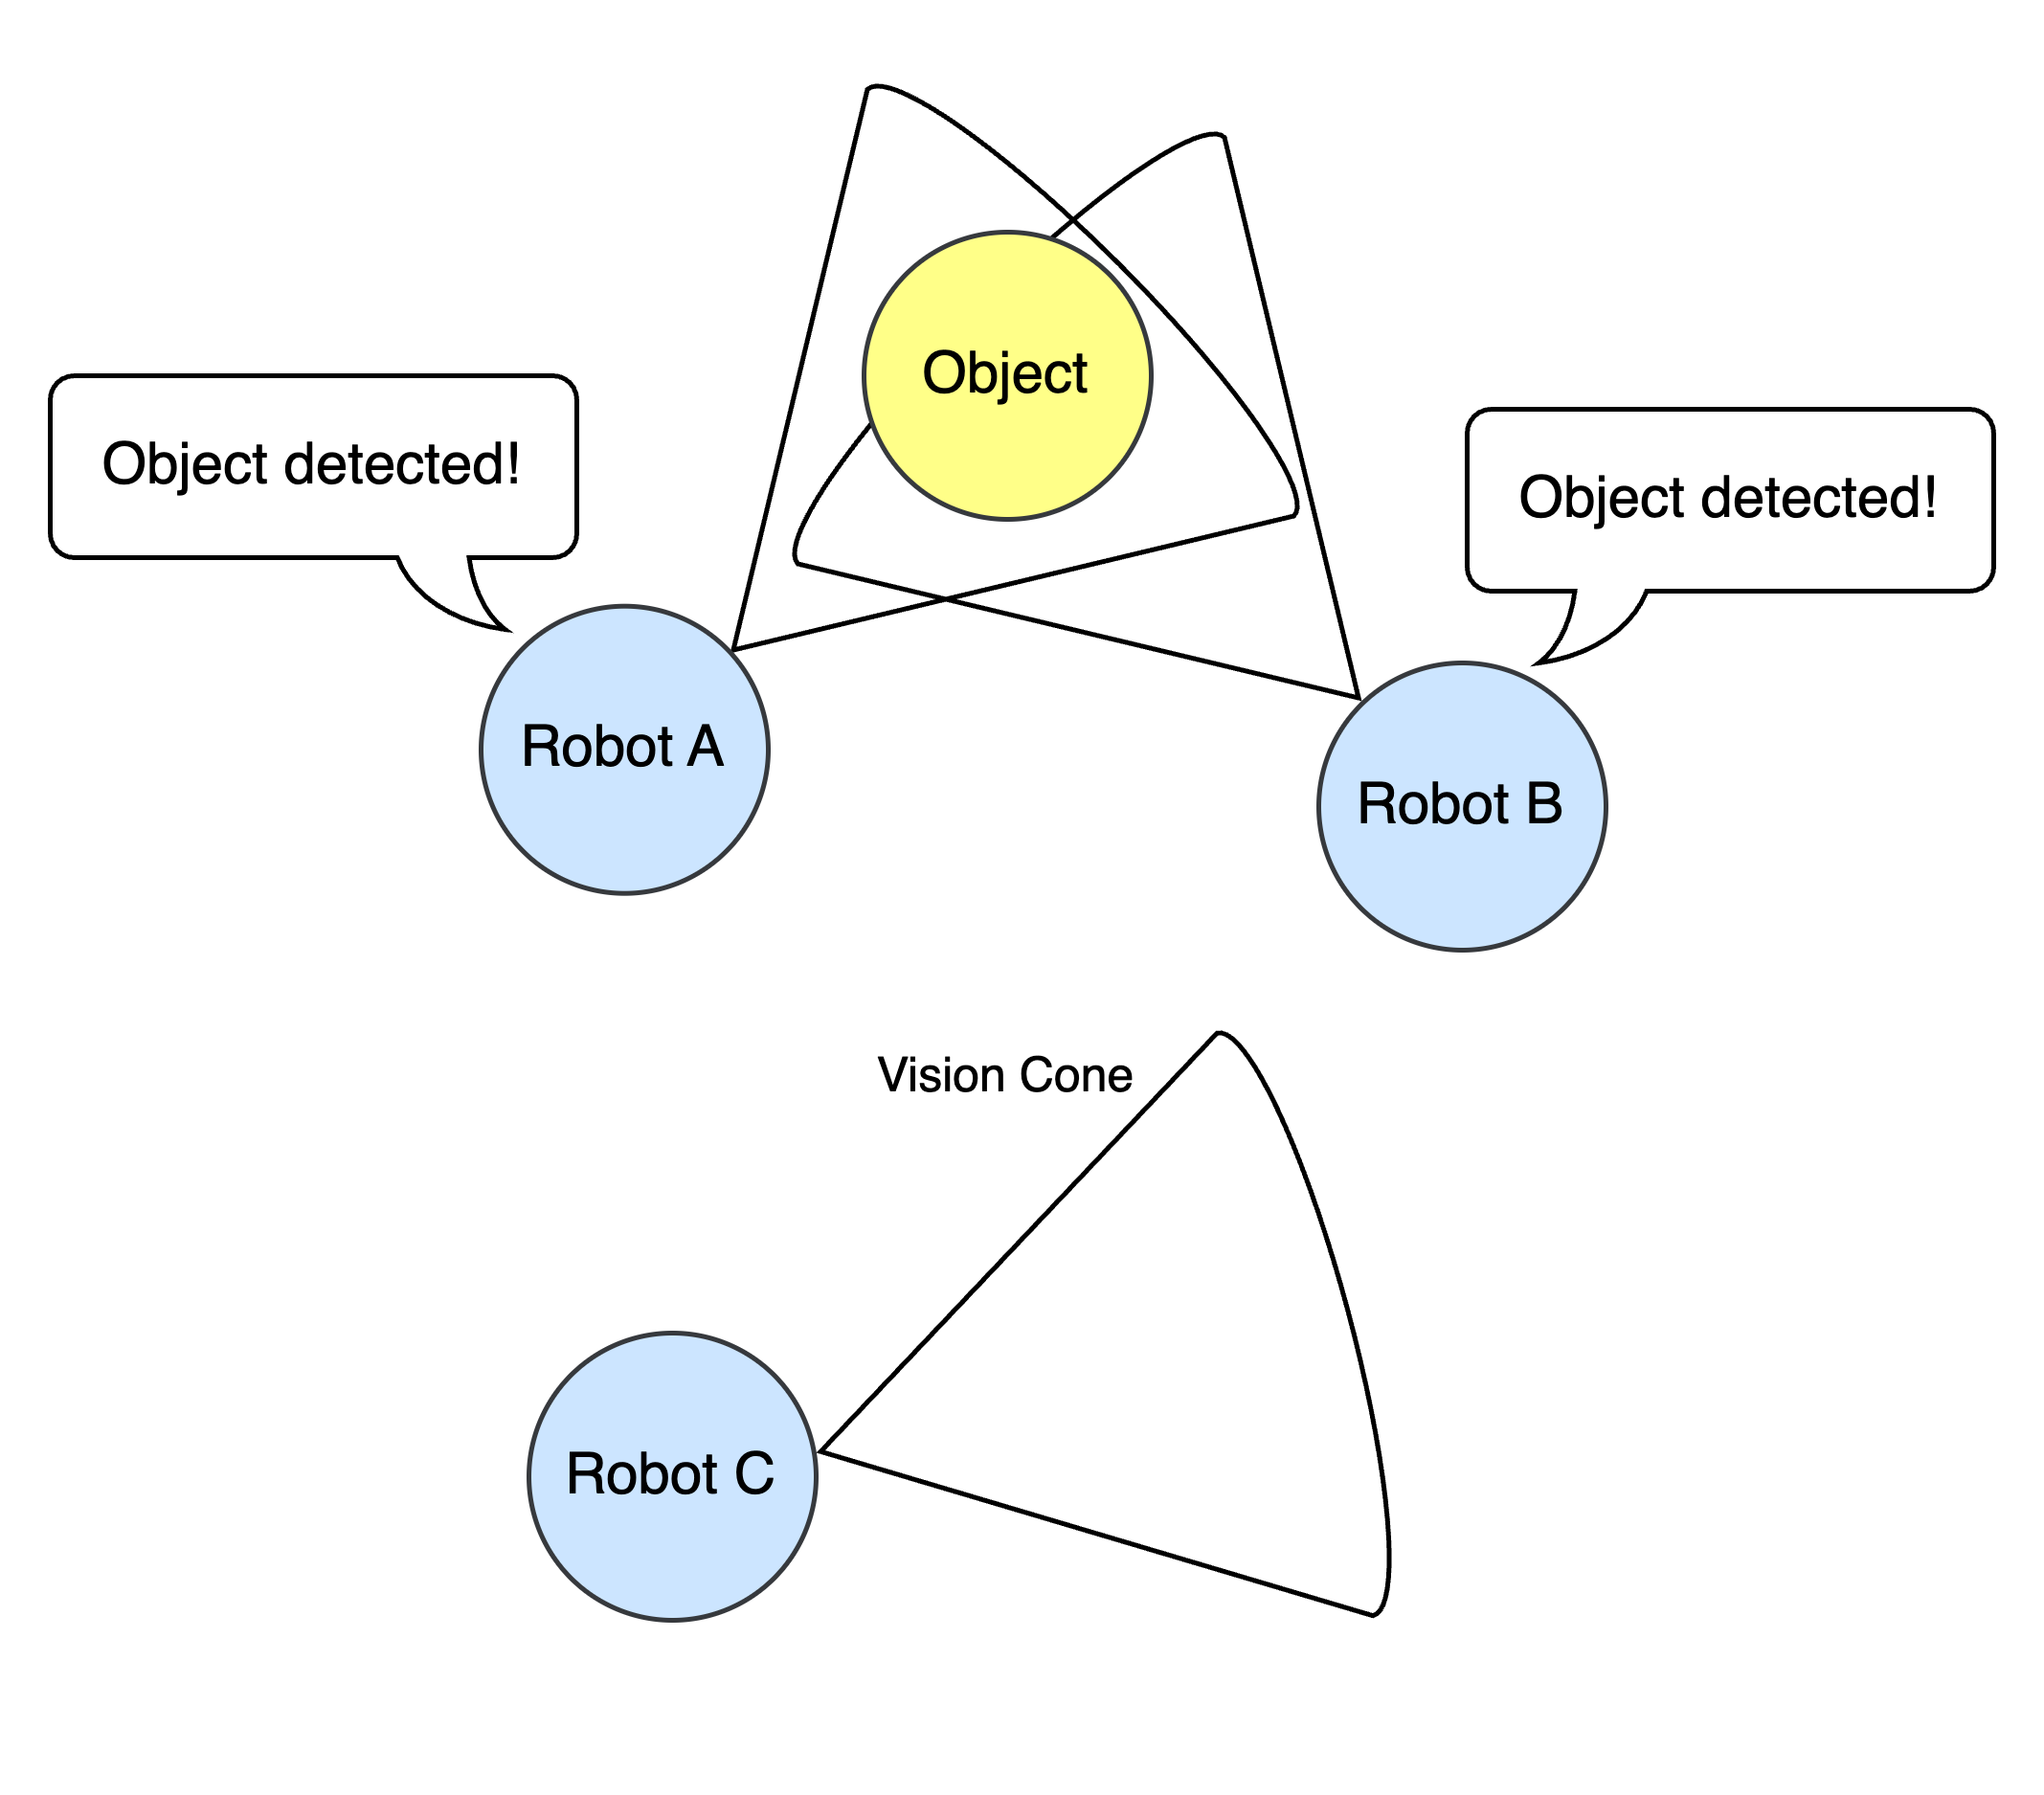
\includegraphics[width=0.6\linewidth]{assets/images/communication/swarm-detection-task-flow-conflict.png}
    \caption{Swarm Detection Task Flow -- Conflict}
    \label{fig:swarm-detection-task-conflict}
\end{figure}

\paragraph*{}
Since there is a claiming mechanism to become the taskmaster in charge of path computations, it is imperative to design communication in such a way that any \textit{conflicting claims} in the exact moment are handled appropriately. An instance of \textit{conflicting claims} is when multiple robots detect the object at the same time, hence claiming to become the taskmaster, similarly to the situation portrayed in \ref{fig:swarm-detection-task-conflict}. The handler of this situation is the designed \textbf{consensus algorithm} for the swarm. Figure \ref{fig:consensus-algorithm} outlines the underlying mechanism of the consensus algorithm.

\begin{figure} [H]
    \centering
    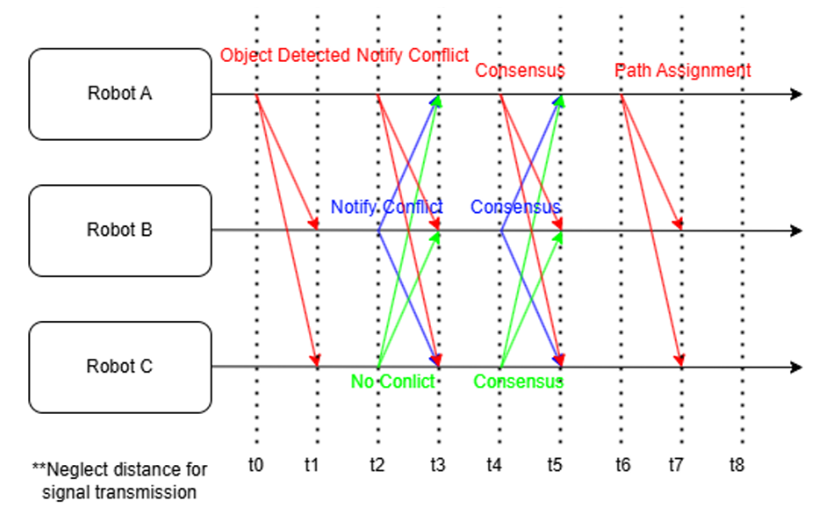
\includegraphics[width=0.9\linewidth]{assets/images/communication/consensus.png}
    \caption{Consensus Algorithm}
    \label{fig:consensus-algorithm}
\end{figure}

\paragraph*{}
The consensus algorithm functions by referring to a \textit{priority queue} once conflicting claims are observed. This priority queue determines the taskmaster by appointing the claimant with the higher priority the taskmaster role. Subsequently, the claimant is repositioned to the end of the priority queue for future claims to partially decentralize the operation. An account of this consensus mechanism is when Robot A and Robot C detect an object at the same time, with Robot C being higher on the priority queue. Robot C will get the taskmaster assignment for that particular detection, then rearranged to the end of the priority queue. If Robot A and Robot C detect an object at the same instance again, Robot A will receive the role, and also gets rearranged to the end of the queue. After the taskmaster assignment resolution is complete, the \textit{swarm detection task flow} will occur as designed.

\paragraph*{}
The swarm communication approaches, particularly the \textit{constant coordinate stream}, are primarily required to help robots efficiently utilize resources and avoid collisions, especially during random movement when no objects have been detected. The \textit{swarm detection task flow} is designed to efficiently travel to designated coordinates in order to prepare for collective movement of the detected object by gripping. The consensus algorithm is also designed to allow seamless coordination and eliminate potential conflicts in the swarm communication.
